\chapter{Diseño e implementación} % Main chapter title

\label{Chapter3} % Change X to a consecutive number; for referencing this chapter elsewhere, use \ref{ChapterX}

En este capítulo se detalla el diseño de la arquitectura del sistema en todos sus componentes. Se menciona el motivo de la elección de cada caso y la implementación correspondiente.

%----------------------------------------------------------------------------------------
%	SECTION 1
%----------------------------------------------------------------------------------------

\section{Cadena de procesamiento de inteligencia artificial}
\label{sec:cadenaProcesamiento}

En esta sección se detalla la implementación de los modelos de inteligencia artificial utilizados en la plataforma \textit{Google Colaboratory (Colab)}.

\subsection{Arquitectura}

La arquitectura de la cadena de procesamiento se compone de tres modelos de inteligencia artificial:

\begin{itemize}
\item Modelo detector de objetos Yolo, cuyos pesos pre-entrenados se obtuvieron de la página de DarkNet \citep{YOLO_MODELO}.
\item Modelo seguidor de objetos Deepsort, cuyos pesos pre-entrenados se obtuvieron de un repositorio \citep{DEEPSORT_MODELO}.
\item Manejo extractor de características Osnet, cuyos pesos pre-entrenados se obtuvieron de la librería Torchreid \citep{OSNET_MODELO}.
\end{itemize}

Cada uno de estos modelos se encuentran conectados en serie entre sí generando una cadena, como se observa en la figura \ref{fig:cadenaProcesamiento}.

\begin{figure}[ht]
	\centering
	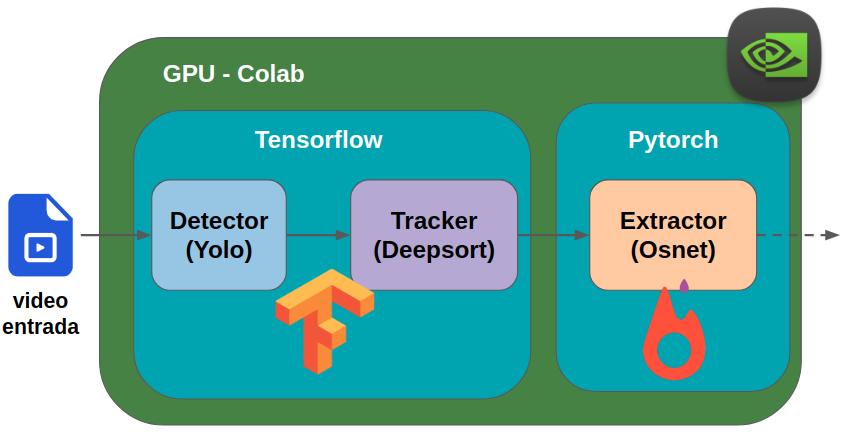
\includegraphics[scale=.50]{./Figures/cadenaProcesamiento.png}
	\caption{Cadena de procesamiento de inteligencia artificial.}
	\label{fig:cadenaProcesamiento}
\end{figure}

Para poder utilizar estos modelos es necesario contar con las siguientes librerías:
\begin{itemize}
\item Python versión 3.7 o superior.
\item Tensorflow GPU versión 2.3.1.
\item Pytorch versión 1.8.
\end{itemize}


\subsection{Integración de los modelos}

Cada modelo en la cadena realiza un aporte al sistema de detección y seguimiento de personas. Por cada frame que transcurre del video se realiza el siguiente proceso:

\begin{itemize}
\item El detector recibe la imagen entera del frame y por cada persona encontrada retorna una caja que la representa. Esa caja está conformada por sus coordenadas respecto a su ubicación en la imagen original (top, left, bottom ,right) y el grado de certeza de detección (score).
\item El seguidor recibe  el vector de cajas de personas y a cada una de ellas le asigna un identificador único (id), que representa a cada persona en seguimiento.
\item El extractor recibe el vector de cajas y personas en seguimiento y genera por cada una de ellas un vector de características. Los vectores obtenidos simbolizan a cada persona en ese frame.
\end{itemize}

En la figura \ref{fig:aporteModelos} se observa el aporte de cada modelo en la cadena de procesamiento.

\begin{figure}[ht]
	\centering
	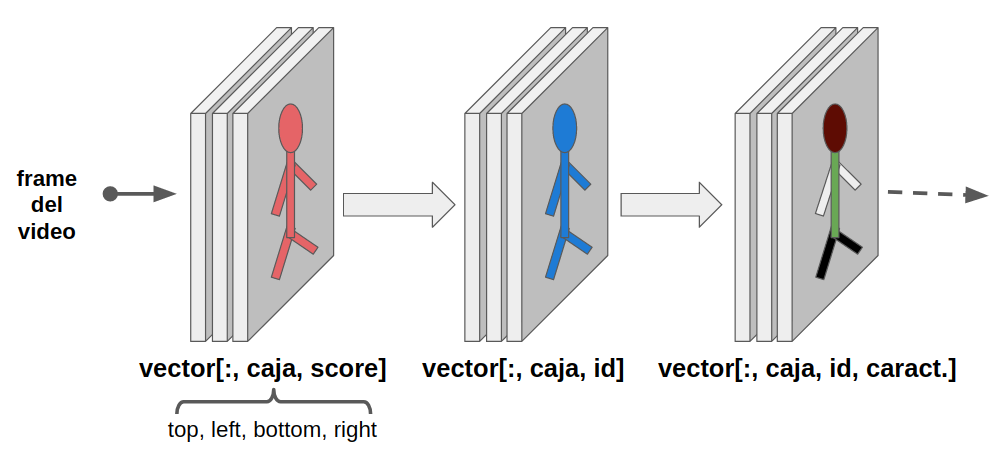
\includegraphics[scale=.50]{./Figures/aporteModelos.png}
	\caption{Integración de los modelos.}
	\label{fig:aporteModelos}
\end{figure}

\newpage

En la figura \ref{fig:aporteModelos2} se observa al detalle como la información se transforma desde el frame capturado por el video hasta llegar al final de la cadena. Cada modelo se utiliza como una caja independiente cuya salida está representada por un vector de datos, con formato compatible con el siguiente modelo en la cadena.

\begin{figure}[ht]
	\centering
	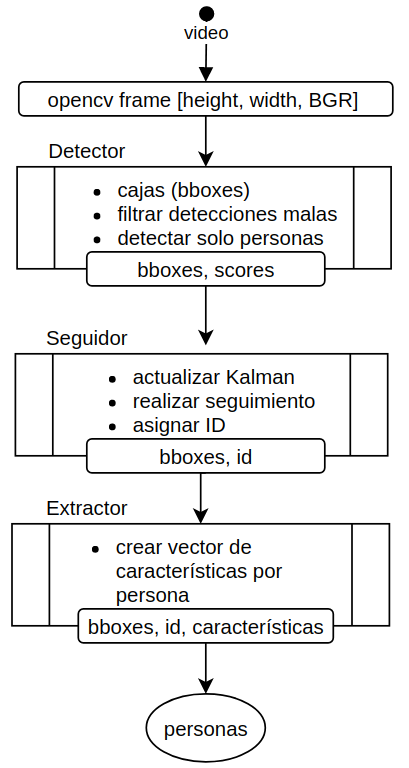
\includegraphics[scale=.75]{./Figures/aporteModelos2.png}
	\caption{Detalle de la cadena de procesamiento.}
	\label{fig:aporteModelos2}
\end{figure}

\newpage

%----------------------------------------------------------------------------------------
%	SECTION 2
%----------------------------------------------------------------------------------------

\section{Entrenamiento de un modelo basado en Osnet}
\label{sec:entrenamientoOsnet}

En esta sección se detalla la selección del dataset, la preparación de los datos y el entrenamiento de un extractor de características basado en la arquitectura del modelo Osnet.

\subsection{Preparación de datos}

Existen diversos datasets disponibles \citep{DATASETS} para entrenar modelos de clasificación y extracción de características de personas. Para la elaboración de este trabajo se optó por utilizar el dataset ``RPIfield'' \citep{RPIfield}, el cual está autorizado para su libre uso y con el consentimiento de los participantes para el entrenamiento de este tipo de modelos.

El dataset RPIfield está formado por capturas de 112 personas en 12 cámaras, en las cuales al menos cada individuo aparece en tres cámaras distintas. En la figura \ref{fig:capturasDataset} se observa un ejemplo de las capturas disponibles en este dataset.

\begin{figure}[ht]
	\centering
	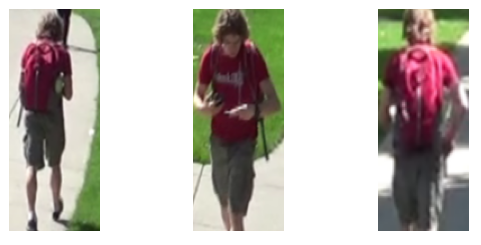
\includegraphics[scale=.70]{./Figures/capturasDataset.png}
	\caption{Capturas disponibles del dataset RPIfield.}
	\label{fig:capturasDataset}
\end{figure}

\subsubsection{Composición del dataset}

Dentro de la carpeta del dataset se encuentra la carpeta "Data", dentro de la cual hay 12 subcarpetas (una por cada cámara). Dentro de cada una hay una o varias carpetas por persona (por id), por ejemplo con el id 1:
\begin{itemize}
\item Las capturas de la primera vez que aparece la persona en una cámara se almacenan en la carpeta ``1''.
\item Si vuelve a aparecer en la misma cámara en capturas posteriores, estas aparecerán en la carpeta ``1\_1''.
\end{itemize}

Este patrón se repite "N" veces por cada id en cada cámara según la cantidad de veces que reaparecieron. Las capturas están almacenadas como un archivo \file{.png} de tamaño variable (aproximadamente 200 x 100 píxeles). En el nombre de la imagen se encuentra el número de frame de la captura.

\newpage

\subsubsection{Distribución de los datos}

El dataset original cuenta con 211644 capturas. En la figura \ref{fig:distribucionOriginal} se observa como se encuentran distribuidas entre los 112 participantes.

\begin{figure}[ht]
	\centering
	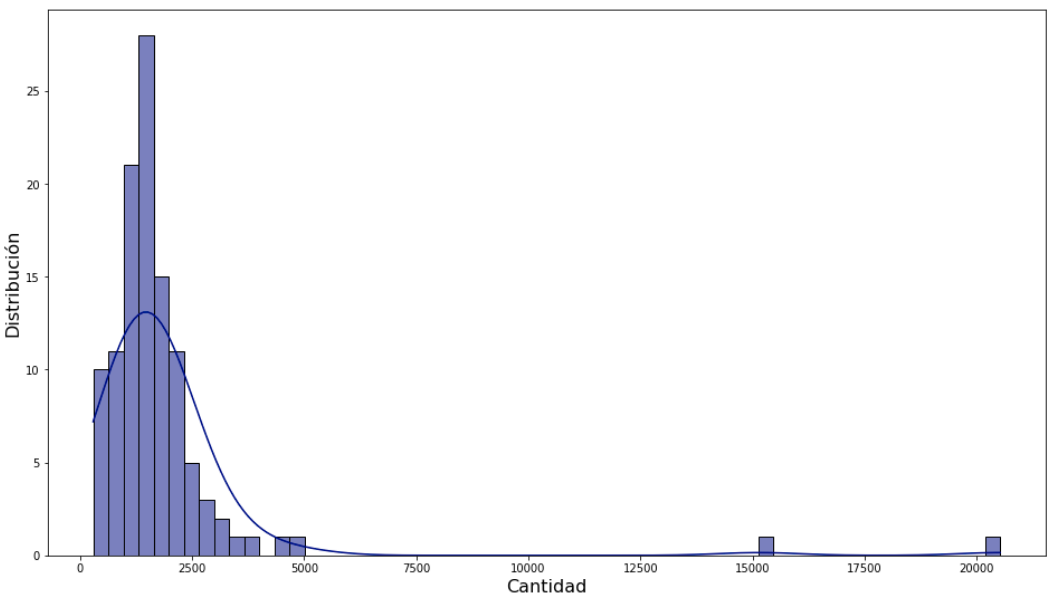
\includegraphics[scale=.50]{./Figures/distribucionOriginal.png}
	\caption{Distribución del dataset original.}
	\label{fig:distribucionOriginal}
\end{figure}

Del análisis de los datos obtenidos del dataset original se desprende que:
\begin{itemize}
\item La cantidad de capturas promedio por persona es 1890.
\item La cantidad de capturas del cuantil 5\% es 540.
\item La cantidad de capturas del cuantil 95\% es 3357.
\item El desvió estándar de capturas por persona es 2325.
\end{itemize}

A fin de balancear el dataset se decidió tomar menos capturas de las personas más frecuentes (aquellas que superan el cuantil 95\%) ya que por lo observado en los datos poseen muchas imágenes repetidas que no aportan valor al sistema.

\subsubsection{Transformación de los datos}

Con el objetivo de balancear el dataset se realizaron dos tipos de procesamiento de datos:
\begin{itemize}
\item Submuestreo de aquellas personas que superan el cuantil 95\% (un total de 6 personas).
\item Aumento de datos de aquellas personas debajo del 80\% de la media (un total de 23 personas).
\end{itemize}

Dado que las imágenes son de baja resolución y definición, no es posible aplicar una gran distorsión sin que se pierda información. La única técnica de aumento de datos que se utilizó fue duplicar las muestras menos frecuentes creando una copia de cada imagen espejada horizontalmente. En la figura \ref{fig:distribucionFinal} se observa la distribución del dataset modificado.

\newpage

\begin{figure}[ht]
	\centering
	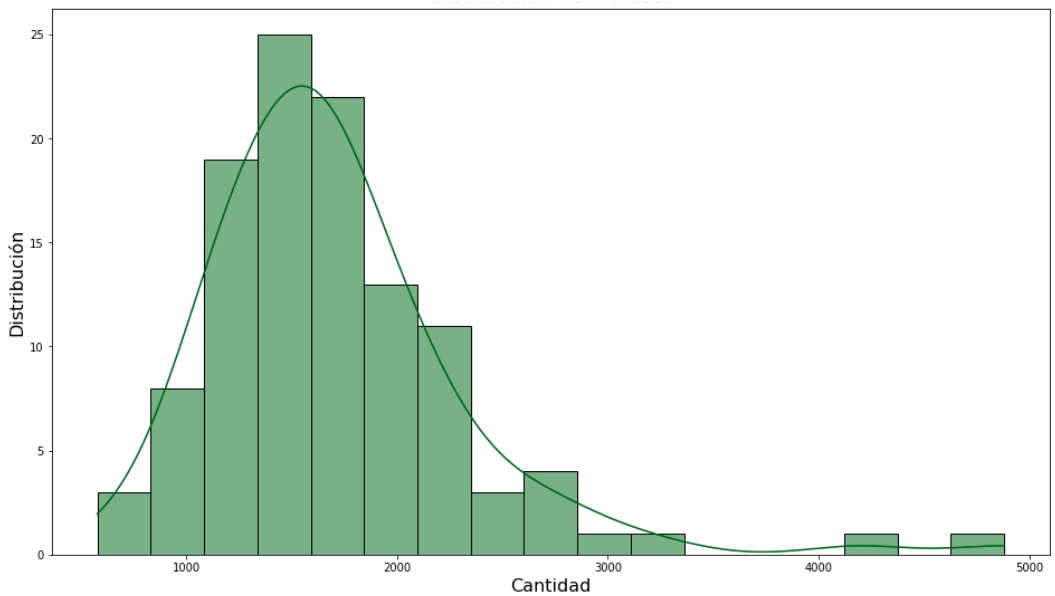
\includegraphics[scale=.50]{./Figures/distribucionFinal.png}
	\caption{Distribución del dataset modificado.}
	\label{fig:distribucionFinal}
\end{figure}

El dataset modificado posee una distribución de datos más balanceada y pareja que el original, como se ilustra en la tabla \ref{tab:datasets}.

\begin{table}[h]
	\centering
	\caption[Dataset]{Comparación de datasets.}
	\begin{tabular}{l c c c}    
		\toprule
		\textbf{Dataset}   & \textbf{Cantidad [cap.]} & \textbf{Promedio [cap.]} & \textbf{Desvió estándar [cap.]}\\
		\midrule
		Original & 211644 & 1890   & 2325 \\		
		Modificado & 173599 & 1600  & 620 \\
		\bottomrule
		\hline
	\end{tabular}
	\label{tab:datasets}
\end{table}

El dataset modificado posee menos capturas que el dataset original, aún así la cantidad es suficiente para entrenar un modelo de clasificación de imágenes. De las 173599 capturas se reservaron 140055 imágenes para entrenamiento (80\%), 15799 para validación (9\%) y 17745 para evaluación (11\%).

\newpage

\subsection{Entrenamiento grueso y fino}

El entrenamiento del modelo basado en Osnet se dividió en dos etapas: el entrenamiento grueso y fino. En ambas etapas se utilizó el dataset modificado y el entorno de Colab aprovechando los recursos de GPU que la plataforma provee. El consumo de los datos durante el entrenamiento se efectuó con la herramienta \textit{ImageDataGenerator}\ de la librería Keras.

\subsubsection{Entrenamiento grueso}

El entrenamiento grueso partió del uso de un modelo basado en Osnet con sus pesos pre-entrenados con el dataset de ImageNet \citep{IMAGENET}, un dataset público utilizado para entrenar modelos de clasificación de imágenes. Basado en los pesos pre-entrenados se aplicó la técnica de \textit{transfer learning}\ congelando las capas inferiores del modelo y sustituyendo las capas superiores acorde al dataset ``RPIfield'', como se observa en la figura \ref{fig:entrenamientoGrueso}.

\begin{figure}[ht]
	\centering
	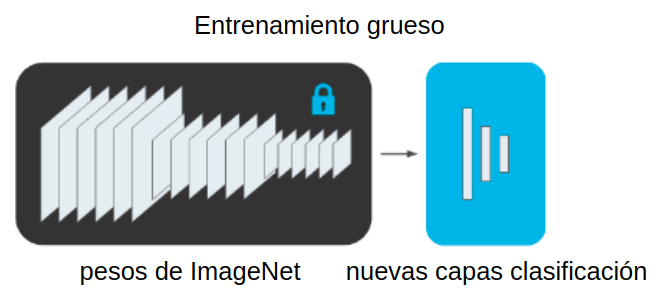
\includegraphics[scale=.60]{./Figures/entrenamientoGrueso.png}
	\caption{Entrenamiento grueso.}
	\label{fig:entrenamientoGrueso}
\end{figure}

Se entrenó el modelo en diez iteraciones durante 40 minutos con una tasa de aprendizaje de 0,001, en la figura \ref{fig:entrenamientoGruesoResultado} se observa que la exactitud alcanzada por el modelo durante el entrenamiento grueso es de aproximadamente 60\%.

\begin{figure}[ht]
	\centering
	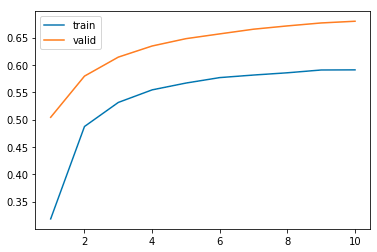
\includegraphics[scale=1.]{./Figures/entrenamientoGruesoResultado.png}
	\caption{Resultado del entrenamiento grueso.}
	\label{fig:entrenamientoGruesoResultado}
\end{figure}

\newpage

\subsubsection{Entrenamiento fino}

El entrenamiento fino partió del uso del modelo utilizado en la sección anterior. Esta vez se entrenaron todas las capas del modelo utilizando una tasa de aprendizaje más baja a fin de realizar un ajuste fino, como se observa en la figura \ref{fig:entrenamientoFino}.

\begin{figure}[ht]
	\centering
	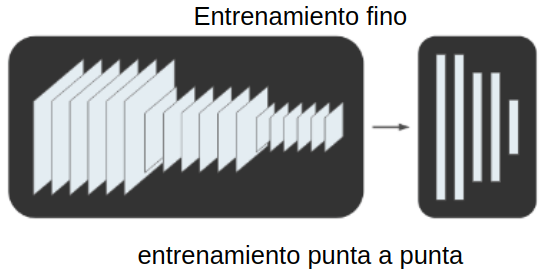
\includegraphics[scale=.60]{./Figures/entrenamientoFino.png}
	\caption{Entrenamiento fino.}
	\label{fig:entrenamientoFino}
\end{figure}

Se entrenó el modelo en trece iteraciones durante tres horas con una tasa de aprendizaje de 0,00001. En la figura \ref{fig:entrenamientoFinoResultado} se observa que la exactitud alcanzada por el modelo durante el entrenamiento fino es de aproximadamente 93\%.

\begin{figure}[ht]
	\centering
	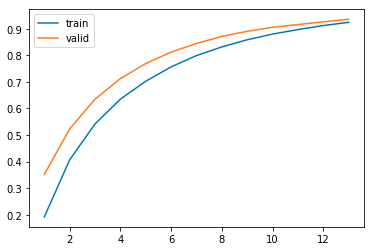
\includegraphics[scale=1.]{./Figures/entrenamientoFinoResultado.png}
	\caption{Resultado del entrenamiento fino.}
	\label{fig:entrenamientoFinoResultado}
\end{figure}

Como última instancia de validación del entrenamiento, se calcularon las métricas de precisión balanceada \citep{BalancedAccuracy} y precisión promedio \citep{mAP}, como se ilustra en la tabla \ref{tab:metricasEntrenamiento}.

\begin{table}[h]
	\centering
	\caption[Métrica Entrenamiento]{Métricas de entrenamiento.}
	\begin{tabular}{l c}    
		\toprule
		\textbf{Métricas}   & \textbf{Resultado [\%]} \\
		\midrule
		Exactitud & 93\% \\
		Precisión balanceada & 92\% \\
		Precisión promedio [mAP] & 97\% \\
		\bottomrule
		\hline
	\end{tabular}
	\label{tab:metricasEntrenamiento}
\end{table}

\newpage

\subsection{Comparativa de los diferentes modelos de extracción de características}
\label{sec:comparativaExtractores}

Con el propósito de comparar el extractor de características entrenado (al que llamaremos Cosnet) se armó una galería de imágenes de personas de cuatro videos diferentes, como se observa en la figura \ref{fig:galerias}.

\begin{figure}[ht]
	\centering
	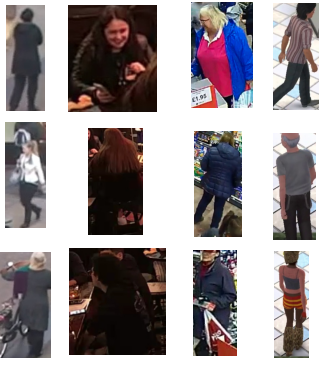
\includegraphics[scale=0.9]{./Figures/galerias.png}
	\caption{Imágenes capturadas para comparar los modelos.}
	\label{fig:galerias}
\end{figure}

Se sometió a ensayo al modelo Osnet (el modelo original), al modelo Cosnet (elaborado en este trabajo) y al modelo DeepMar (mencionado en la sección \ref{sec:exactorOsnet}). Se utilizó la métrica de la silueta \citep{METRICA_SILUETA} para comparar estos modelos, la cual se obtiene como el cociente entre la distancia de todos los puntos de un mismo cluster al centro y la distancia de un cluster con otros. En la figura \ref{fig:metricaSilueta} se observa que cuanto más cerca se encuentren los puntos pertenecientes a un mismo cluster (A) y más alejados estén los clusters entre sí (B), más alta será la métrica de la silueta.

\begin{figure}[ht]
	\centering
	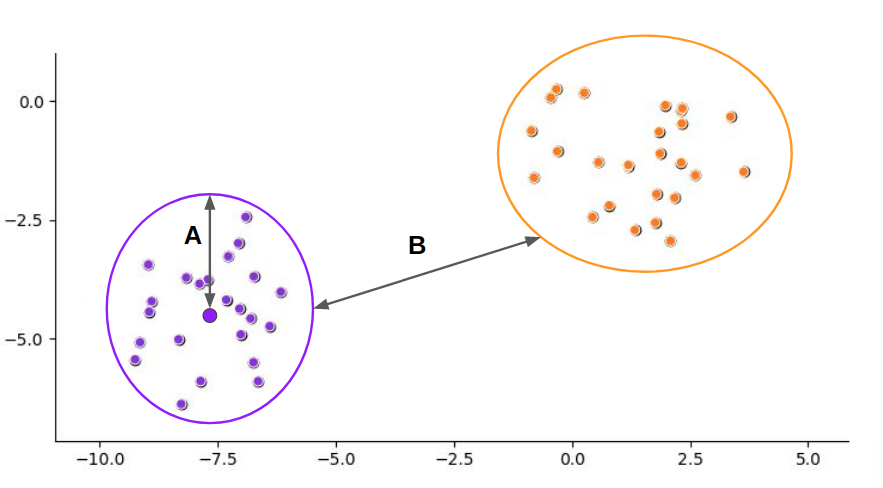
\includegraphics[scale=.5]{./Figures/metricaSilueta.png}
	\caption{Métrica de la silueta.}
	\label{fig:metricaSilueta}
\end{figure}

\newpage

En la figura \ref{fig:comparacionExtractores} se observa que el modelo original de Osnet obtuvo mejor resultado que Cosnet. Este último supera los resultados obtenidos del modelo DeepMar, y por lo tanto, se puede concluir que los procesos de entrenamiento y pre-procesamiento fueron exitosos.

\begin{figure}[ht]
	\centering
	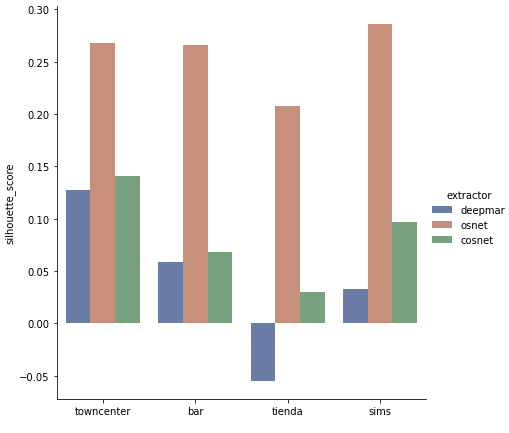
\includegraphics[scale=1.]{./Figures/comparacionExtractores.png}
	\caption{Métrica de la silueta.}
	\label{fig:comparacionExtractores}
\end{figure}

El modelo Osnet tuvo un mejor desempeño porque fue entrenado con la función de pérdida \textit{triple-loss}, que maximiza la distancia entre clusters distintos. En un futuro trabajo se continuará desarrollando el entrenamiento de Cosnet con triple-loss.

\newpage

%----------------------------------------------------------------------------------------
%	SECTION 3
%----------------------------------------------------------------------------------------

\section{Manejo de oclusiones y re-identificación}
\label{sec:oclusionesReID}

En esta sección se detalla el uso del extractor de características para solucionar problemas en el seguimiento y monitoreo de personas. Se describen las técnicas de re-identificación utilizadas y la validación de las mismas.

\subsection{Segmentación de personas}
\label{sec:segmentacionPersonas}

La segmentación es el proceso por el cual se separa un conjunto de datos por similitud o características en grupos llamados clusters. El proceso de segmentación es un éxito cuando los clusters representan correctamente los datos y no hay solapamiento entre ellos.

A fin de representar a las personas como un conjunto de datos, se utiliza el modelo extractor de características que produce un vector por cada individuo. Los vectores, de 512 dimensiones, se utilizan para segmentar a las personas y transformarlas en clusters.

En la figura \ref{fig:clusterPersonas} se observa como las capturas de una persona forman un cluster, agrupando sus características. Se utilizó la técnica de \textit{Nearest Centroid} \citep{NEAREST_CENTROID} para calcular el centro de cada cluster dado el conjunto de vectores que lo conforman.

\begin{figure}[ht]
	\centering
	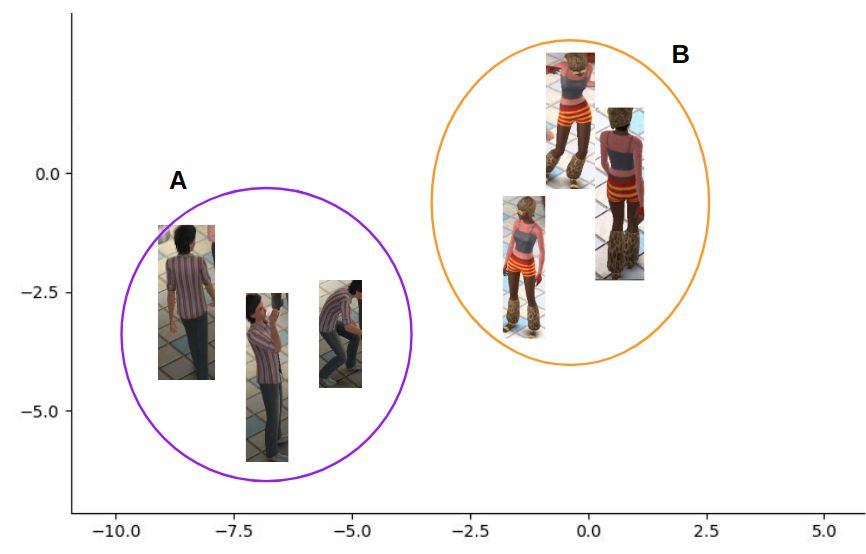
\includegraphics[scale=.6]{./Figures/clusterPersonas.jpg}
	\caption{Segmentación de personas en clusters.}
	\label{fig:clusterPersonas}
\end{figure}

Finalmente cada cluster formado en el sistema representará a una persona con un identificador único denominado \textit{cluster id}. A medida que la persona incorpora más vectores a su cluster más se robustece y mejor la representa.

\newpage

\subsection{Re-identificación por vectores}

El proceso de re-identificación de personas busca relacionar una nueva persona por su vector de características con un cluster ya conformado. El objetivo es mantener el seguimiento de una persona con el mismo cluster, es decir con el mismo identificador, a pesar de que se haya salido de escena por unos segundos. Para poder calcular la similitud entre el vector de una persona y los diferentes clusters se utiliza la similitud coseno \citep{COSINE_SIMILARITY}, la cual retorna un valor entre -1 y 1 siendo 1 la expresión para máxima similitud.

En la figura \ref{fig:similitudCoseno} se observa que dado un punto verde que representa el vector de una nueva persona, se calcula la similitud coseno ``A'' y ``B''. En este caso, el resultado del proceso será que el nuevo vector es más probable que pertenezca al cluster ``A'' que al cluster ``B'', y por lo tanto, la nueva persona será asociada con el cluster ``A''.

\begin{figure}[ht]
	\centering
	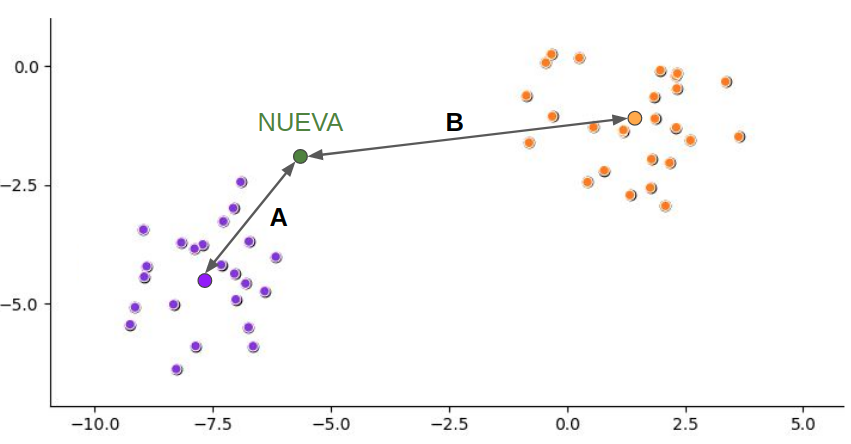
\includegraphics[scale=.6]{./Figures/similitudCoseno.png}
	\caption{Re-identificación por similitud coseno.}
	\label{fig:similitudCoseno}
\end{figure}

Esta técnica no contempla casos de falsos positivo, es decir, asociar erróneamente una persona con un cluster que no le pertenece. En la próxima sección se discute como se utiliza este principio para mejorar el sistema de seguimiento de personas.

\subsection{Mejora del seguimiento por vectores}

Durante el monitoreo de una persona pueden ocurrir diferentes problemas relacionados con oclusiones o intercambios de identificador como se detalla en la sección \ref{sec:desafiosSeguimiento}. En estos casos, lo que sucede es que se pierde el identificador de seguimiento o se intercambia por uno erróneo, y el sistema debe reaccionar para re-identificar a la persona con su correspondiente cluster. 

\newpage

El sistema para mejorar el seguimiento por vectores utiliza dos estrategias:
\begin{itemize}
\item \textit{Matching}: proceso por el cual el sistema intenta asociar un cluster disponible a un persona que presente un identificador de seguimiento desconocido, es decir, uno nuevo para el sistema. Este proceso puede concluir en que la persona que apareció en escena es un individuo nuevo que no se había detectado hasta el momento (se genera un nuevo cluster), o concluir que en realidad es una persona que se estaba monitoreando pero desapareció de escena (se la asocia con un cluster existente).
\item \textit{Mismatching}: proceso por el cual el sistema evalúa constantemente si una persona en monitoreo realmente pertenece al cluster asociado. Este proceso busca encontrar identificadores que hayan sido intercambiados por culpa de una oclusión. El proceso concluye en la búsqueda de los clusters correctos para aquellas personas que no hayan pasado la prueba.
\end{itemize}

El sistema de mejora está conformado por una serie de \textit{thresholds} y \textit{timers} a fin de evitar generar falsos positivos. Estos valores de configuración se obtuvieron de forma teórica utilizando matrices de similitud, y se ensayaron de forma empírica en diferentes condiciones y escenarios a fin de validar los parámetros seleccionados.

En la figura \ref{fig:matrizSimilitud} se observa la matriz de similitud que se obtuvo de los personajes de ``Los Sims''. En promedio, la similitud entre clusters para este escenario fue de 0,66. El mismo proceso se repitió con otros videos y escenarios con el objetivo de estimar los parámetros de configuración del sistema de matching y mismatching.

\begin{figure}[ht]
	\centering
	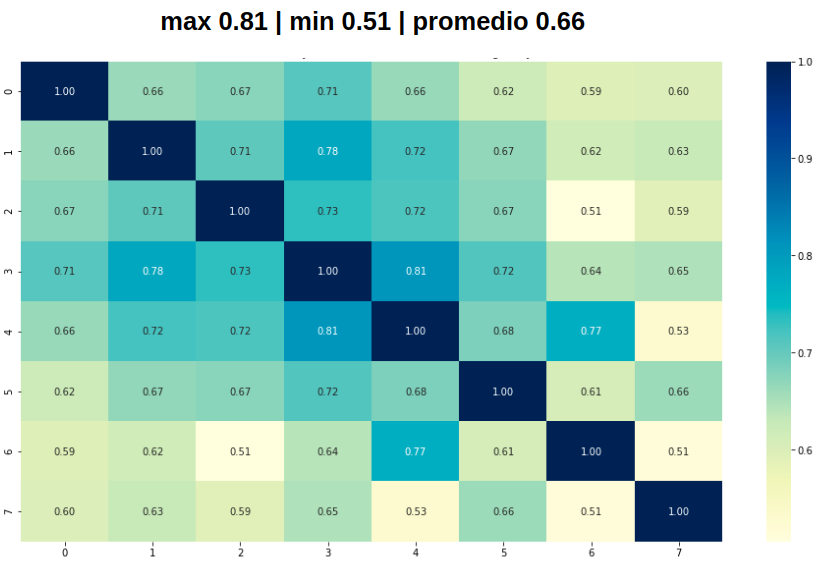
\includegraphics[scale=.65]{./Figures/matrizSimilitud.png}
	\caption{Matriz de similitud de ``Los Sims''.}
	\label{fig:matrizSimilitud}
\end{figure}

\newpage

\subsection{Validación del manejo de oclusiones y re-identificación}

Con el propósito de validar el sistema re-identificación por características se creó una serie de herramientas que permiten visualizar como se aplica la estrategia de matching o mismatching durante el procesamiento de un video.

\subsubsection{Validación de matching}

La estrategia de matching se desencadena cuando aparece una persona con un nuevo identificador de seguimiento y se analiza si pertenece a un cluster disponible, es decir, no utilizado actualmente por otra persona en escena. En la figura \ref{fig:validarMatching} se observa un ejemplo de una persona nueva que entra en escena con identificador ``52'' (persona de remera gris de caja color violeta). El sistema asocia a esta persona con el cluster disponible número 2.

\begin{figure}[ht]
	\centering
	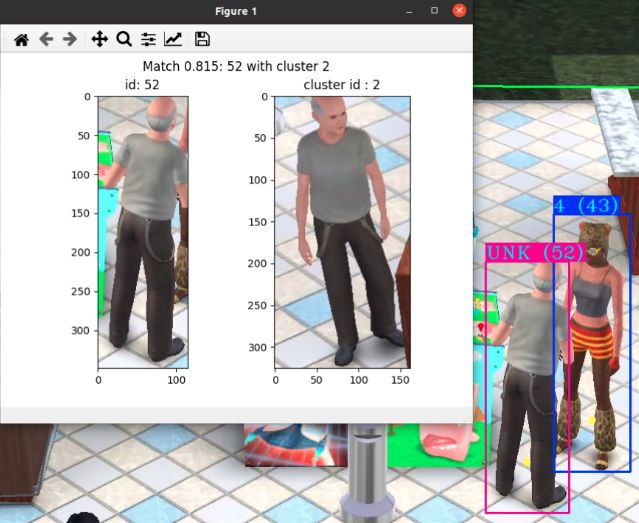
\includegraphics[scale=.7]{./Figures/validarMatching.jpg}
	\caption{Validación de la estrategia de matching.}
	\label{fig:validarMatching}
\end{figure}

La herramienta de validación arroja una ventana con los datos que el sistema posee en ese momento para aplicar la estrategia de matching. En este caso, la herramienta indica que el sistema encontró un cluster candidato para la persona con identificador ``52'' con un 81.5\% de confianza. La validación de matching se la considera exitosa si la foto de la persona nueva coincide con la última foto capturada por el cluster recomendado para ella. 

En caso de no coincidir las imágenes significa que el sistema no debía ejecutar la estrategia de matching, y por lo tanto, se lo considera un falso positivo. Como existen falsos positivos en el sistema, el objetivo es reducirlos al máximo y alcanzar los requerimientos de precisión de monitoreo establecidos para este trabajo.

\newpage

\subsubsection{Validación de mismatching}

La estrategia de mismatching se desencadena cuando el vector de una persona no coincide durante un determinado tiempo con el cluster asociado, es decir, la similitud coseno se encuentra por debajo del parámetro configurado. En la figura \ref{fig:validarMismatching} se observa un ejemplo en donde el hombre de remera gris captura la caja con identificador ``43'' que pertenecía a la mujer que lo acompaña.

\begin{figure}[ht]
	\centering
	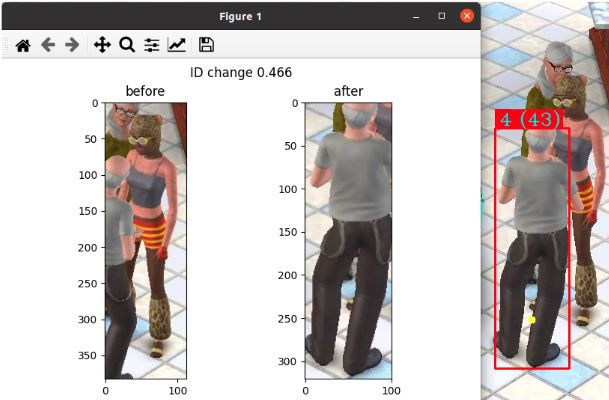
\includegraphics[scale=.7]{./Figures/validarMismatching.jpg}
	\caption{Validación de la estrategia de mismatching.}
	\label{fig:validarMismatching}
\end{figure}

La herramienta de validación arroja una ventana con los datos que el sistema posee en ese momento para aplicar la estrategia de mismatching. En este caso, la herramienta indica que el sistema encontró una persona cuyo vector de características coincide tan solo un 46.6\% respecto al cluster asociado con identificador ``4''. La validación de mismatching se la considera exitosa si la foto de la persona de la derecha no coincide con la captura del cluster asociado a ella que se encuentra a la izquierda.

En caso de coincidir las imágenes significa que el sistema no debía ejecutar la estrategia de mismatching, y por lo tanto, se lo considera un falso positivo. Existen falsos positivos cuando una persona cambia drásticamente su apariencia fuera de escena y es confundida con una persona nueva o distinta.

\newpage

%----------------------------------------------------------------------------------------
%	SECTION 4
%----------------------------------------------------------------------------------------

\section{Motor de seguimiento y monitoreo (Engine)}
\label{sec:engine}

En esta sección se detalla el diseño del sistema de manejo de oclusiones, re-identificación de personas, incorporación de zonas de interés y cálculo de métricas. De ahora en adelante se hará mención a este sistema bajo el nombre de \textit{Engine}.

\subsection{Arquitectura}

El objetivo principal del Engine es recibir las detecciones, identificadores y características de salida de la cadena de procesamiento de inteligencia artificial para mejorar el sistema de seguimiento y monitoreo. En la figura \ref{fig:arquitecturaEngine} se observan las distintas etapas que componen al Engine.

\begin{figure}[ht]
	\centering
	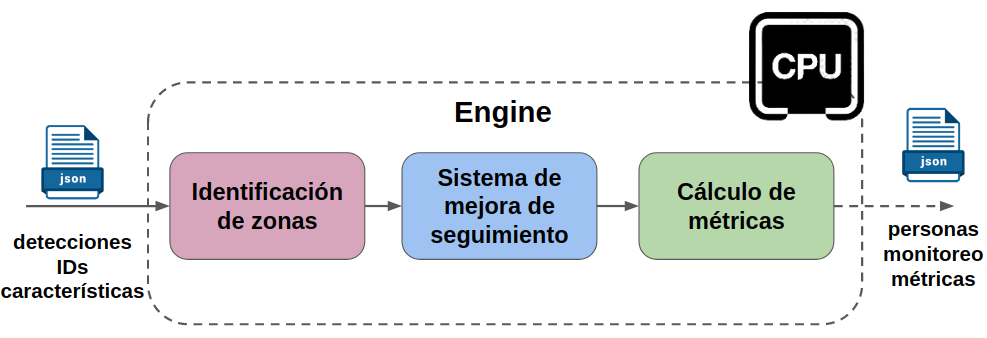
\includegraphics[scale=.5]{./Figures/arquitecturaEngine.png}
	\caption{Arquitectura del Engine.}
	\label{fig:arquitecturaEngine}
\end{figure}

A continuación se detalla la funcionalidad de cada etapa de la figura \ref{fig:arquitecturaEngine}:
\begin{itemize}
\item Identificación de zonas: esta etapa es la encargada de determinar en que zona se encuentra cada una de las detecciones, utilizando como dato las zonas definidas por el usuario en la interfaz web. Se utilizan algoritmos geométricos \citep{POLYGON_TEST_INSIDE} para determinar si la detección se encuentra contenida dentro del polígono que define la zona de interés.
\item Sistema de mejora de seguimiento: esta etapa posee la heurística que integra el uso de las detecciones y las características para el manejo de oclusiones y re-identificación, mejorando la calidad de seguimiento y monitoreo. La heurística está conformada por una máquina de estados que se explica en la sección \ref{sec:maquinaEstados}.
\item Cálculo de métricas: esta etapa recibe las personas en monitoreo del sistema de mejora de seguimiento y calcula las métricas de cada una y su interacción con las zonas de interés. El resultado de esta etapa es un conjunto en datos en formato \textit{JSON (JavaScript Object Notation)} que captura la interfaz web para presentar al usuario los resultados.
\end{itemize}

\newpage

\subsection{Máquina de estados}
\label{sec:maquinaEstados}

La máquina de estados del sistema de monitoreo integra algoritmos de aprendizaje automático y segmentación con el objetivo de mejorar el seguimiento de las personas. Utiliza técnicas de manejo de oclusión y re-identificación de personas dividas en los estados que se observan en la figura \ref{fig:maquinaEstados}.

\begin{figure}[ht]
	\centering
	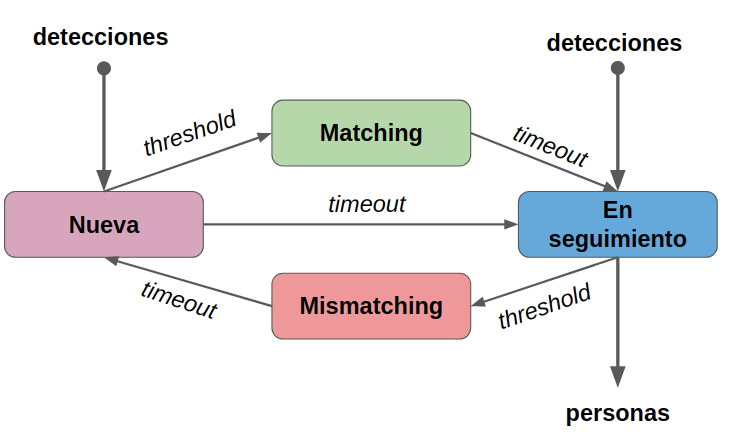
\includegraphics[scale=.6]{./Figures/maquinaEstados.png}
	\caption{Máquina de estados del Engine.}
	\label{fig:maquinaEstados}
\end{figure}

Los datos de entrada al sistema son las detecciones, que ingresarán al estado ``nueva'' o ``en seguimiento'' en función de si el identificador de seguimiento es nuevo para el sistema o no. Todas aquellas personas con identificador ya reconocidos tienen asignadas un cluster y por lo tanto son consideradas personas en monitoreo.

A continuación se detalla la lógica de la máquina de estados.
\begin{itemize}
\item Nueva: estado en el cual ingresan las nuevas detecciones y se analiza si es posible aplicar la estrategia de matching, es decir, relacionar una nueva detección con un cluster disponible (re-identificación). En el caso de que fuera posible aplicar la estrategia (el threshold es válido) el estado pasa a ``matching''. En el caso de no poder asociar la detección con una persona registrada, la nueva detección pasa al estado ``en seguimiento'' y se crea un cluster nuevo.
\item En seguimiento: estado en el cual ingresan las personas asociadas con un cluster y por lo tanto en monitoreo. Si la similitud de una persona en seguimiento respecto a su cluster disminuye por debajo del threshold, el sistema pasa a estado de ``mismatching'' para evaluar esa persona.
\item Matching: estado en el cual se mantiene en observación una persona candidata de re-identificación. En caso de sostenerse el estado por encima del tiempo de timeout, el estado de esa persona pasa a ``en seguimiento''.
\item Mismatching: estado en el cual se mantiene en observación una persona que no coincide con las características de su cluster. En caso de sostenerse el estado por encima del tiempo de timeout, el estado de esa persona pasa a ``nueva'', rompiendo el vínculo entre esa detección y su cluster asociado.
\end{itemize}

\newpage

%----------------------------------------------------------------------------------------
%	SECTION 5
%----------------------------------------------------------------------------------------

\section{Interfaz de usuario}
\label{sec:gui}

La interfaz de usuario es la aplicación web que se utiliza para configurar las zonas de interés en el recinto y observar la evolución de las métricas y el monitoreo de personas. Para el desarrollo de esta aplicación se utilizaron las siguientes tecnologías:
\begin{itemize}
\item Flask 2.0: \textit{microframework} \citep{FLASK} de Python utilizado para el desarrollo del \textit{back end} e integración con el \textit{front end}.
\item HTML, CSS, Javascript: lenguajes de programación utilizados para el desarrollo del front end.
\end{itemize}

Toda la aplicación funciona dentro del microframework de Flask, en donde, se capturan las solicitudes de usuario por \textit{API REST (Representational 
State Transfer)} \citep{API_REST} y se envían los datos en tiempo real del monitoreo de personas por \textit{websockets} \citep{WEBSOCKETS} a la interfaz de usuario. En la figura \ref{fig:arquitecturaWebApp} se observa la arquitectura de la aplicación web.

\begin{figure}[ht]
	\centering
	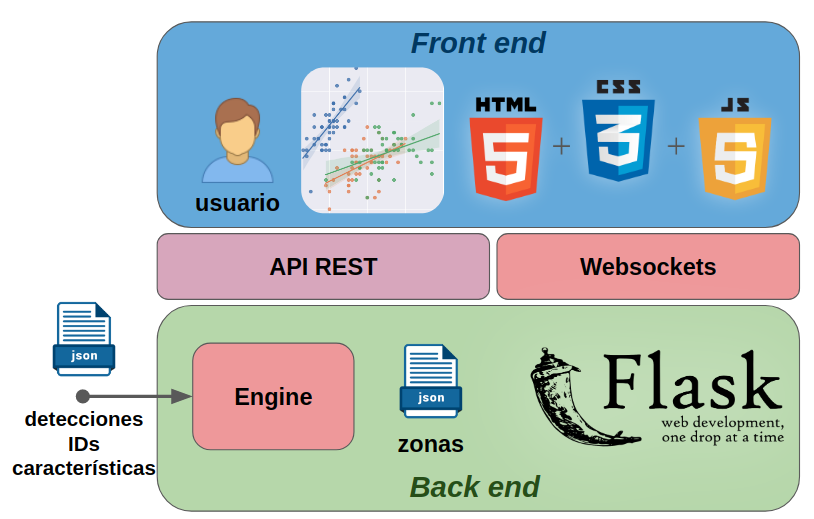
\includegraphics[scale=.6]{./Figures/arquitecturaWebApp.png}
	\caption{Arquitectura de la aplicación web.}
	\label{fig:arquitecturaWebApp}
\end{figure}

El Engine es un proceso que ejecuta la aplicación, utilizando las configuraciones de usuario y los datos obtenidos de la cadena de procesamiento de inteligencia artificial. A medida que los datos son procesados en el Engine se presentan las métricas en la interfaz en diferentes gráficos que se detallarán en las próximas secciones.

\newpage

\subsection{Definición de zonas de interés}
\label{sec:definicionZonasInteres}

Las zonas son definidas como polígonos sobre la imagen del recinto, utilizando el mouse para agregar puntos y formar cada polígono. Para poder agregar un polígono es necesario primero indicar que tipo de zona se desea crear y con qué nombre se la mencionará en la interfaz. Las zonas de interés las define el usuario en el menú de ``Zones''. Hay diferentes tipos de zonas ya pre-definidas en el sistema:

\begin{itemize}
\item \textit{Region Of Interest}: utilizada para delimitar la región de interés, es decir, el área en donde se desea detectar personas. Toda detección que se encuentre fuera de esta zona será descartada.
\item \textit{Avoid}: utilizada para delimitar espacios en donde no se desea detectar personas. Es lo contrario a la ``Region Of Interest'' y se utiliza especialmente para descartar zonas problemáticas.
\item \textit{Entrance}: utilizada para delimitar el espacio de entrada al recinto.
\item \textit{Transit}: utilizada para delimitar espacios en donde las personas pueden transitar de un espacio del recinto a otro sin abandonarlo. Se utiliza para detectar personas que cambian de ambiente, salen de cámara (se pierde la detección), pero el sistema sabe que la persona no ha abandonado el recinto.
\item \textit{Analytics 1/2/3}: utilizada para delimitar espacios genéricos de interés, como por ejemplo: espacio de bebidas, juegos, descanso, etc.
\end{itemize}

En la figura \ref{fig:visualizacionZonas} se observa el ejemplo de algunas zonas dibujadas, se puede apreciar una zona de comida en verde y una zona de tránsito en amarillo.

\begin{figure}[ht]
	\centering
	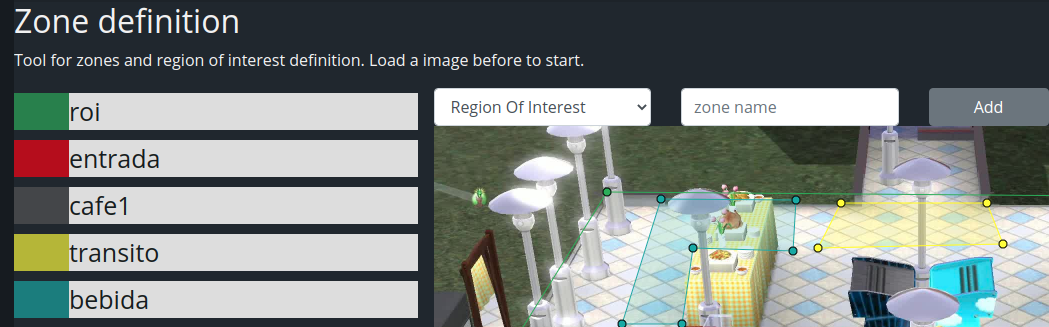
\includegraphics[scale=.5]{./Figures/visualizacionZonas.png}
	\caption{Zonas de interés.}
	\label{fig:visualizacionZonas}
\end{figure}

Cada zona agregada se almacena con su tipo, color y nombre junto con los puntos que conforman al polígono. Estos datos luego se utilizan en el Engine para determinar los espacios transitados por las personas.

\newpage

\subsection{Visualización del seguimiento}

La visualización del monitoreo de personas en tiempo real se encuentra en el menú de ``Test''. La interfaz no muestra a las personas tal cual son vistas por la cámara, sino que genera figuras geométricas para representarlas en la aplicación. En la figura \ref{fig:visualizacionSeguimiento} se observa como son representadas las personas en la interfaz web.

\begin{figure}[ht]
	\centering
	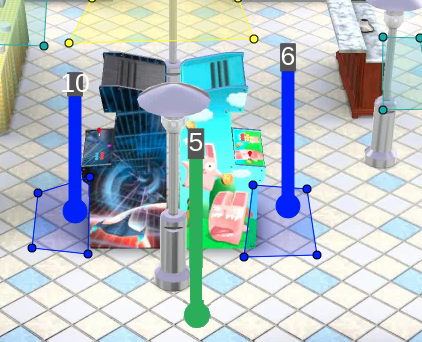
\includegraphics[scale=.8]{./Figures/visualizacionSeguimiento.png}
	\caption{Visualización del monitoreo de personas en tiempo real.}
	\label{fig:visualizacionSeguimiento}
\end{figure}

Cada persona es representada por un poste que en la parte superior muestra el identificador de monitoreo de esa persona. A su vez, el poste se pinta del color de la zona donde la persona es detectada. En la \ref{fig:visualizacionSeguimiento} se observan dos personas que se encuentran en la zona de juegos (azul) y una persona que se encuentra dentro de la región de interés (verde).

\subsection{Visualización de las métricas}

La visualización de las métricas de monitoreo de personas se encuentra en el menú de ``Metrics''. El sistema provee dos tipos de métricas que puede observar el usuario:

\begin{itemize}
\item Tabla ordenada por las zonas de interés más transitadas: tabla que puede utilizar el usuario para ver a golpe de vista cuál fue el área más popular del recinto, como también observar el nivel de interacción de cada zona relativa a otras.
\item Mapa de calor del recinto: gráfico que arroja información acerca de cómo transitaron las personas por el lugar y los espacios en donde más se detuvieron. El usuario puede utilizar este gráfico para observar como las personas transitan de un espacio a otro, lo que le permite optimizar el flujo de tránsito.
\end{itemize}

En la sección \ref{sec:resultados} se detallan ejemplos de métricas y gráficos obtenidos utilizando la interfaz con videos de personas.